a. Apply the RBF-PS method to solve the heat equation and Helmholtz equation (eigenvalue problem for the
Laplacian) in 1D. (The relevant material is Chapter 42-43 in Fasshauer).\\

b. Describe the RBF-PS method in 2D (the implementation is optional).\\\\

\begin{solution}\renewcommand{\qedsymbol}{}\ \\

    a. For the implementation here, we take the work that we did previously and instead of solving for
    the coeeficients using our RBF matrix, we use this matrix as a differentiation matrix. So, we will
    solve the system:
    
    $$(A'' A^{-1})u=u_t$$
    
    where $A''$ is the matrix $A$ using the second derivative of the RBF instead of the RBF itself.
    Solving the heat equation $u_t=u_{xx}$, we have the following code using a myriad of conditions.
    
    \begin{center}
        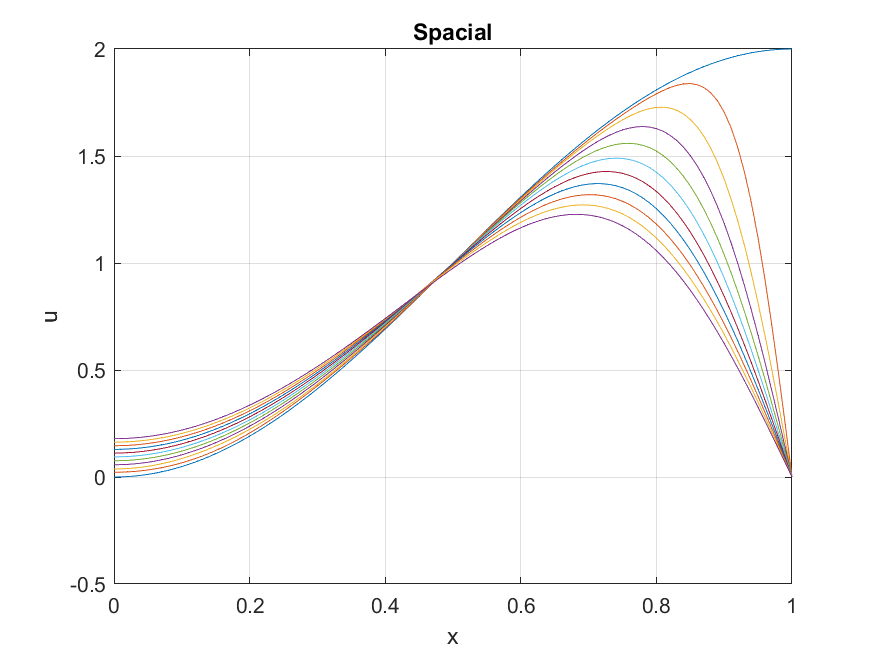
\includegraphics[scale=0.5]{problem3aheatx.png}
        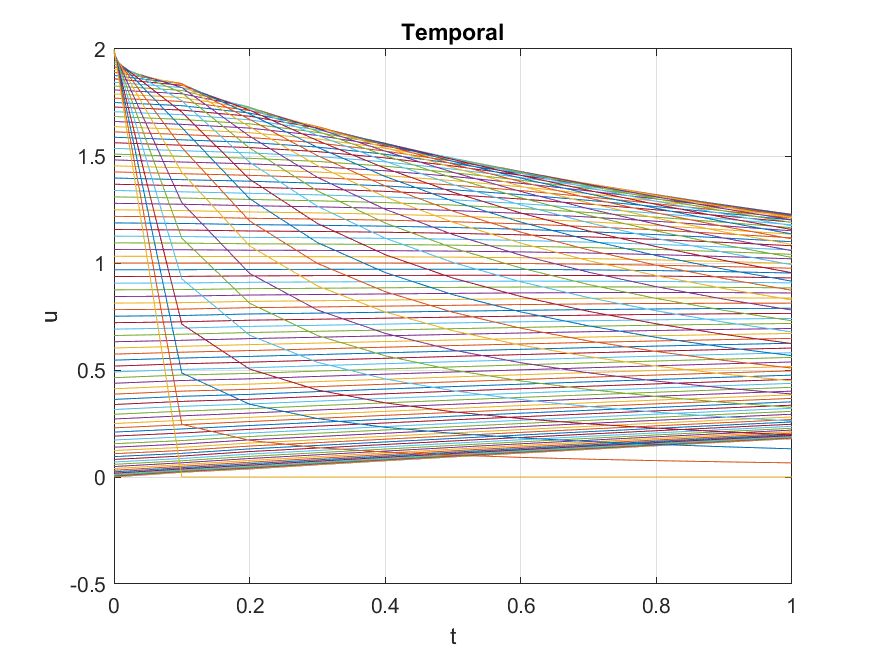
\includegraphics[scale=0.5]{problem3aheatt.png}
        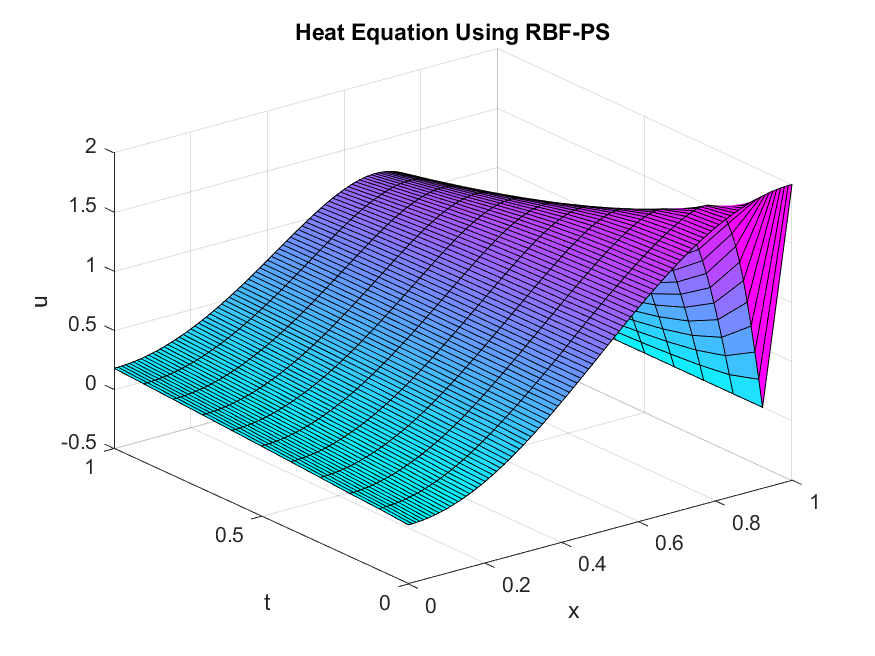
\includegraphics[scale=0.5]{problem3aheat.png}
        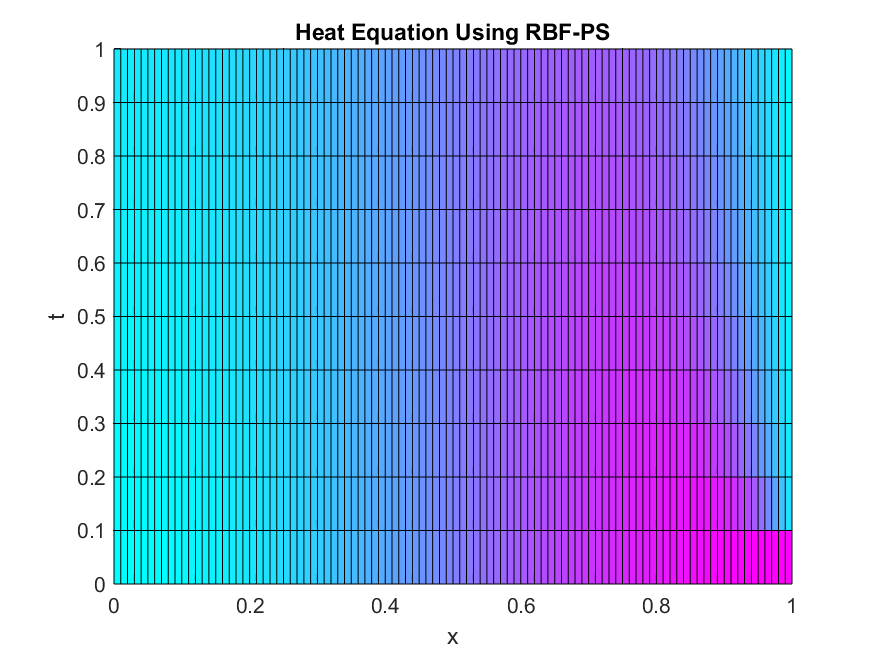
\includegraphics[scale=0.5]{problem3aheat2d.png}
    \end{center}

    Now, for the Helmholtz equation, we more or less use the same kind of code. The major difference is
    that we instead focus our attention to the eigenvalue problem rather than solving a particular
    equation or system. So, we use the code below.

    \begin{center}
        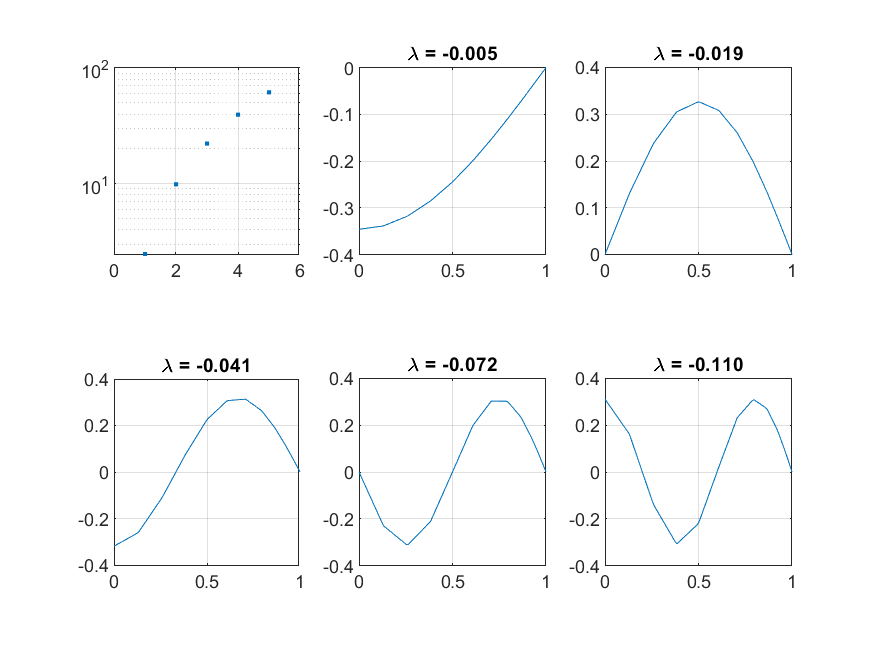
\includegraphics[scale=0.8]{problem3ahelm.png}
    \end{center}

\pagebreak

    b. To do this in the 2 dimensional case, we would need to look back at our work in spectral methods
    in 2D.

\end{solution}

\newpage
\lstinputlisting{problem3aheat.m}
\newpage
\lstinputlisting{problem3ahelm.m}